\documentclass{beamer}
\usepackage[brazilian]{babel}
\usepackage[utf8]{inputenc}
\usepackage[T1]{fontenc}
\usepackage{minted}
\usepackage{algorithmic}
\usepackage[brazilian]{algorithm}
\usepackage{amsthm}
\usemintedstyle{tango}
\usepackage{graphicx}

\renewcommand{\algorithmicrequire}{\textbf{Entrada:}}
\renewcommand{\algorithmicensure}{\textbf{Saída:}}
\renewcommand{\algorithmicend}{\textbf{fim}}
\renewcommand{\algorithmicif}{\textbf{se}}
\renewcommand{\algorithmicthen}{\textbf{então}}
\renewcommand{\algorithmicelse}{\textbf{else}}
\renewcommand{\algorithmicelsif}{\algorithmicelse\ \algorithmicif}
\renewcommand{\algorithmicendif}{\algorithmicend\ \algorithmicif}
\renewcommand{\algorithmicfor}{\textbf{para}}
\renewcommand{\algorithmicforall}{\textbf{para todos}}
\renewcommand{\algorithmicdo}{\textbf{faça}}
\renewcommand{\algorithmicendfor}{\algorithmicend}
\renewcommand{\algorithmicwhile}{\textbf{enquanto}}
\renewcommand{\algorithmicendwhile}{\algorithmicend}
\renewcommand{\algorithmicloop}{\textbf{loop}}
\renewcommand{\algorithmicendloop}{\algorithmicend\ \algorithmicloop}
\renewcommand{\algorithmicrepeat}{\textbf{repita}}
\renewcommand{\algorithmicuntil}{\textbf{enquanto}}
\renewcommand{\algorithmicprint}{\textbf{imprima}}
\renewcommand{\algorithmicreturn}{\textbf{retorne}}
\renewcommand{\algorithmictrue}{\textbf{verdadeiro}}
\renewcommand{\algorithmicfalse}{\textbf{falso}}


\renewcommand{\theFancyVerbLine}{
  \sffamily\textcolor[rgb]{0.5,0.5,0.5}{\scriptsize\arabic{FancyVerbLine}}}

\AtBeginSection{\frame{\sectionpage}}
\newtranslation[to=brazilian]{Section}{Se\c c\~ao}

\newtheorem{mydef}{Defini\c c\~ao}

\title{PCS730 - Prova}
\author{Lucas Virgili}
\date{}

\begin{document}

\begin{frame}[fragile]
  \titlepage
\end{frame}


\begin{frame}[fragile]
  \frametitle{1. Introdu\c c\~ao e conceitos b\'asicos}
  \begin{itemize}
  \item \textbf{Slides 1.20 - 1.21}\\
    Os slides acima descrevem, em ``alto n\'ivel'', os passos
    executados pelo compilador durante o processo de compila\c c\~ao,
    que funcionam como um ``pipeline''.\\

    Inicialmente, \'e necess\'ario que o compilador consiga acessar o
    arquivo-fonte fisicamente, para poder, ent\~ao, acess\'a-lo
    atrav\'es de uma forma mais abstrata. De posse dessa represeta\c
    c\~ao l\'ogica do arquivo-fonte, o compilador pode extrair
    caracteres do fonte e alimentar o analisador l\'exico, que extrai
    os \'atomos do c\'odigo. Esses \'atomos s\~ao, ent\~ao, passados
    ao analisador sint\'atico que pode, assim, criar a \'arvore
    sint\'atica abstrata que representa o programa. Essa \'arvore, por
    sua vez, \'e usada como entrada pelo otimizador, que gera uma
    \'arvore reduzida, a qual \'e, finalmente, utilizada pelo gerador
    de c\'odigo para gerar o c\'odigo-objeto.
  \end{itemize}
\end{frame}

\begin{frame}[fragile]
  \frametitle{2. Linguagens formais e aut\^omatos}
  \begin{itemize}
  \item \textbf{Elementos do slide 2.20}\\
    O slide 2.20 descreve os tipos de transi\c c\~ao poss\'iveis em
    aut\^omatos de pilha estruturados.
    \begin{enumerate}
    \item Transi\c c\~oes internas, ou seja, sem chamadas de subm\'aquina:
      \begin{enumerate}
      \item Transi\c c\~oes em vazio, sem consumo de \'atomo, do
        estado $j$ para o estado $k$
      \item Transi\c c\~oes com consumo de \'atomo, tamb\'em do estado
        $j$ para o estado $k$.
      \end{enumerate}
    \item Transi\c c\~oes externas, ou seja, com chamadas de
      subm\'aquina:
      \begin{enumerate}
      \item Chamada de subm\'aquina pela m\'aquina $i$ no estado $j$,
        indo para a subm\'aquina $m$ no estado $0$
      \item Retorno da subm\'aquina $i$ no estado $j$ para a
        subm\'aquina que a chamou, $m$, no estado seguinte dela, no
        caso $n$.
      \end{enumerate}
    \end{enumerate}
  \end{itemize}
\end{frame}

\begin{frame}[fragile]
  \frametitle{4. T\'ecnicas cl\'assicas de an\'alise (b) bottom-up}
  \begin{itemize}
  \item \textbf{Simplifica\c c\~ao de aut\^omatos}\\
    A sequ\^encia de slides 4.18 a 4.28 descrevem a sequ\^encia de
    opera\c c\~oes para simplificar os aut\^omatos. Os passos s\~ao os
    seguintes:
    \begin{enumerate}
    \item Eliminar as transi\c c\~oes em vazio: Se um estado $i$ possui
      transi\c c\~ao em vazio para o estado $j$, removemos a transi\c
      c\~ao de $i$ para $j$ e, para toda transi\c c\~ao de $j$ para
      outros estados $k_n$, criamos uma transi\c c\~ao de $i$ para
      $k_j$ com o consumo de \'atomo correto
    \item Elimina\c c\~ao de estados inating\'iveis: construindo-se
      uma \'arvore de atingibilidade do aut\^omato, a partir do n\'o
      principal, repetindo-se o seguinte processo: para cada estado
      n\~ao atingido ainda de cada folha, acrescentamos uma nova folha
      \`a \'arvore. Quando n\~ao pudermos mais acrescentar novas
      folhas, estados que n\~ao est\~ao na \'arvore n\~ao s\~ao
      ating\'iveis e podem ser removidos.
    \item (Continua no pr\'oximo)
    \end{enumerate}
  \end{itemize}

\end{frame}

\begin{frame}[fragile]
  \frametitle{Cont.}
  \begin{enumerate}
\setcounter{enumi}{2}
  \item Elimina\c c\~ao de n\~ao-determinismos: podem sobrar
      transi\c c\~oes para mais de um estado com o mesmo consumo de
      \'atomo. Para removermos tais transi\c c\~oes, criamos um estado
      auxiliar para cada transi\c c\~ao desse tipo. Tais estados devem
      ter as transi\c c\~oes que ``saem'' dos estados de origem.
  \end{enumerate}
\end{frame}

\begin{frame}
  \frametitle{6. Automatiza\c c\~ao da constru\c c\~ao de compiladores}
  \begin{itemize}
  \item Flex \'e um programa gerador de tokenizers a partir de
    express\~oes regulares e c\'odigo em uma linguagem base, como
    C\footnote{Usar o de SML foi horr\'ivel.}. Podemos us\'a-lo para
    extrair os terminais de um c\'odigo fonte, ou seja, construir
    analisadores l\'exicos com ele.\footnote{Ref.: http://flex.sourceforge.net/}
  \item Bison \'e o equivalente sint\'atico do Flex: ele converte uma
    gram\'atica livre de contexto em um aut\^omato LR. Podemos usar o
    Bison para escrever o reconhedor sint\'atico de uma linguagem.
  \item Podemos usar o par acima para criar um compilador, bastando
    escrever as fun\c c\~oes sem\^anticas na linguagem base para cada
    regra sint\'atica ou
    l\'exica.\footnote{Ref.: http://www.gnu.org/software/bison/}
  \end{itemize}
\end{frame}

\begin{frame}
  \frametitle{7. Recupera\c c\~ao de erros}
  \begin{itemize}
  \item \textbf{Um m\'etodo simples de recupera\c c\~ao de
      erros}\footnote{Note que eu ainda acho que n\~ao se recuperar do
    erro e abandonar o programador com sua incompet\^encia \'e o
    melhor a se fazer}\\
  Uma maneira que eu imagino que seja razoavelmente simples para se
  implementar \'e criar um estado ``lix\~ao''. Todos os estados que
  n\~ao s\~ao o ``lix\~ao'' t\^em transi\c c\~oes para o lix\~ao com
  todos os s\'imbolos que n\~ao representam transi\c c\~oes ``reais'',
  ou seja, as transi\c c\~oes para estados n\~ao lix\~ao.

  J\'a o estado lix\~ao tem apenas duas transi\c c\~oes: uma para
  algum estado inicial com algum dos s\'imbolos que ele sabe consumir
  e outra transi\c c\~ao de ``fecho'', consumindo quaisquer outros
  s\'imbolos. Ou seja, at\'e encontrar o s\'imbolo correto, o estado
  ``lix\~ao'' remove s\'imbolos da entrada.

  A implementa\c c\~ao seria um tanto mon\'otona, contudo, j\'a que
  seria mais simples adicionar o estado lixo na pr\'opria matriz de
  transi\c c\~ao do que na gram\'atica.
  \end{itemize}
\end{frame}

\begin{frame}
  \frametitle{8. Funcionalidades do compilador}
  \begin{itemize}
  \item Grande parte da sem\^antica de um programa n\~ao \'e feita
    pelos componentes mencionados. O compilador deve:
    \begin{itemize}
    \item Manter a tabela de s\'imbolos, o que pode ser feito pelo
      analisador l\'exico;
    \item Atruibuir atributos aos s\'imbolos;
    \item Guardar informa\c c\~oes sobre o escopo;
    \item Representar tipos;
    \item Checar se o uso dos identificadores est\'a correto;
    \item Gerenciar mem\'oria;
    \item Comunica\c c\~ao com o ambiente de execu\c c\~ao.
    \end{itemize}
  \end{itemize}
\end{frame}

\begin{frame}
  \frametitle{9. Formas intermedi\'arias}
  \begin{itemize}
  \item Vantagens:
    \begin{enumerate}
    \item Gera\c c\~ao de c\'odigo objeto especializado para
      diferentes arquiteturas;
    \item V\'arias linguagens diferentes gerando essa linguagem e
      utilizadas ao mesmo tempo;
    \item Otimiza\c c\~oes baseadas nela podem usadas para todas as
      linguagens que geram a linguagem intermedi\'aria.
    \end{enumerate}
  \item Desvantagens:
    \begin{enumerate}
    \item Origem da m\'aquina virtual: \'e c\'odigo-aberto?, quem a
      mant\'em?, uso comercial?, etc.
    \end{enumerate}
  \item N\~ao, pode-se converter essa linguagem intermedi\'aria depois
    para outras diferentes
  \item Diversas formas intermedi\'arias podem ser usadas em conjunto
    quando cada uma facilita algum passo da compila\c c\~ao. Por
    exemplo, uma permite otimiza\c c\~oes locais de forma simples e
    outra permite uma redu\c c\~ao do tamanho do objeto.
  \end{itemize}
\end{frame}

\begin{frame}
  \frametitle{10. An\'alise sem\^antica}
  \begin{itemize}
  \item Sem\^antica est\'atica \'e o ``acochambramento'' feito pelo
    compilador para poder lidar com gram\'aticas dependentes de
    contexto. Nesse caso, \'e de responsabilidade da sem\^antica
    analisar e garantir a correta associa\c c\~ao entre
    identificadores e valores, tipos e etc.
  \item O nome \'e inadequado pois isso deveria ser um aspecto sint\'atico.
  \item Exemplos s\~ao o gerenciamento de mem\'oria, de escopos,
    comunica\c c\~ao com o ambiente de execu\c c\~ao.
  \end{itemize}
\end{frame}

\begin{frame}
  \frametitle{11. Gera\c c\~ao de c\'odigo}
  \begin{itemize}
  \item A arquitetura da LLVM permite isso:
    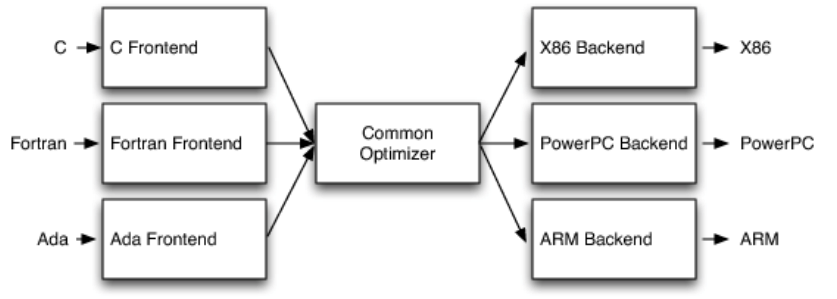
\includegraphics[width=.8\pdfpagewidth]{llvm.png}
  \item Basta criarmos um novo ``filtro'' do c\'odigo intermedi\'ario
    usado pela linguagem que gera c\'odigo objeto para a nova arquitetura.
  \end{itemize}
\end{frame}

\begin{frame}
  \frametitle{12. Otimiza\c c\~ao de c\'odigo}
  \begin{itemize}
  \item Otimiza\c c\~ao global se aplica considerando-se o programa
    como um todo, ao contr\'ario das otimiza\c c\~oes locais, que
    baseiam-se em blocos b\'asicos. Exemplo de global \'e a elimina\c
    c\~ao de regi\~oes inacess\'iveis e de local \'e \emph{tail-call
      recursion}.
  \item Otimiza\c c\~oes depententes de m\'aquina s\~ao as que s\'o
    podem ser feitas (ou t\^em efeito) em determinadas
    arquitetura. Por exemplo, usar alguma instru\c c\~ao de manipula\c
    c\~ao vetorial. J\'a otimiza\c c\~oes indepentes baseiam-se em
    proprieades matem\'aticas do programa, procurando uma representa\c
    c\~ao equivalente por\'em mais eficiente.
  \item Todos estes s\~ao objetivos diferentes de otimiza\c c\~ao:
    quer-se minimizar o tempo de execu\c c\~ao ou o tamanho do
    execut\'avel ou a quantidade de comunica\c c\~ao?
  \item Programas sequenciais podem ser otimizados de forma diferente
    de paralelos, j\'a que funcionam de forma diferente. Por exemplo,
    podemos querer minimizar o n\'umero de acessos \`a mem\'oria
    compartilhada e sincroniza\c c\~ao de caches em um programa
    paralelo, enquanto em um sequencial esses problemas n\~ao
    existem.
  \end{itemize}
\end{frame}
\end{document}